% vim: set spell spelllang=es syntax=tex :

\section{Descripción del framework}

Para aumentar el throughput del sistema se aplicaran las dos técnicas discutidas
con anterioridad. En primer lugar el sistema no estará limitado a tomar solo un
cuadro por ves. La segunda optimización consta en dividir cada cuadro para que
cada parte pueda ser procesada por un thread distinto. También seria deseable
que las distintas pilas de plugins ejecuten de forma independiente una de la
otra para que el retardo de procesamiento de cada cuadro sea menor.  Sin
embargo, en los experimentos realizados se comprobó que el overhead introducido
por el incremento en la cantidad de tareas afecta de forma notable el
rendimiento de la aplicación, por lo cual se opto que las pilas ejecuten de
forma secuencial.

Para esto se propone en primera instancia la siguiente secuencia de
procesamiento para cada ítem (un cuadro en el caso de la solución especifica
para fútbol de robots):

\begin{enumerate}

\setcounter{enumi}{-1}

\item	Antes de la ejecución el usuario establece una cantidad máxima de tareas
	en ejecución simultanea.

\item	El hilo de captura genera o captura un ítem y lo deposita en el buffer.

\item	Una tarea maestra consume el ítem mas reciente del buffer y crea una
	tarea de búsqueda para su procesamiento. Si hay mas tareas que las
	permitidas o no hay ítems en el buffer, espera.

\item	La tarea de búsqueda fracciona el ítem y crea una tarea por cada
	fragmentos creado. Mientras espera no contribuirá al limite de tareas en
	ejecución.

\item	Las tareas procesaran cada fragmento con cada pila de plugins.  Cuando
	la ultima pila termine de procesar el fragmento, lo eliminara.

\item	Cuando se terminan de procesar todos los fragmentos, la tarea de
	búsqueda resume la ejecución para eliminar el ítem de la memoria y
	posiblemente realizar tareas conteo.

\end{enumerate}

Algo que no queda especificado en la descripción anterior, es la naturaleza de
las tareas. Por un lado, las tareas pueden comenzar su ejecución al momento de
ser creadas o pueden esperar a que la cantidad de tareas en ejecución sea menor
que el máximo establecido. La primera opción tiene como desventaja que dado que
el único control sobre la cantidad de tareas se realiza al consumir un ítem, la
cantidad de tareas en ejecución sea mayor al máximo establecido durante una
porción significativa de la duración del programa. La segunda opción solo
funcionara satisfactoriamente si se asegura que la próxima tarea a ejecutar sea
la mas antigua.

El establecer un máximo de hilos en ejecución nos permite asegurarnos de que los
hilos no compitan por la CPU y que esta se mantenga ocupada siempre que haya
tareas a realizar, simplemente estableciendo tal máximo como el números de
procesadores disponibles. Es por esto que la segunda opción es la mas deseable.

TODO: Diagrama del framework

\section{Implementación del framework}

El framework fue implementado en \emph{C++} utilizando \emph{OpenMP}. La,
elección del lenguaje principalmente se debe al deseo de trabajar tomando como
base el desarrollo realizado por Torres en \cite{torres2014}, en especial se
espero hacer uso de los plugins. Por su parte, el autor original del software
eligió este lenguaje debido a su eficiencia y paradigma. Dado que el sistema
debe procesar las cuadros en tiempos acotados, la eficiencia es es crucial,
mientras que el paradigma orientado a objetos permite establecer fácilmente la
interfaz de los plugins. Por otra parte, utilizar \emph{OpenMP} es una
desviación del software original.

\emph{OpenMP} es una API de bibliotecas y directivas al compilador para la
definición de paralelismo de alto nivel para sistemas de memoria compartida en
\emph{C}, \emph{C++} y \emph{Fortran}\cite{ompWeb}. La ventaja de \emph{OpenMP}
es que permite la creación de regiones paralelas, secciones criticas, tareas y
puntos de sincronización, simplemente marcando un bloque de código con unas
pocas directivas al compilador.

Las clases del framework básico son las siguientes:

\begin{description}

\item[Item:] Esta clase define un tipo genérico de los ítems que serán tratados
	por el sistema.

\item[RingBuffer:] Este es el buffer donde se guardan los ítems generados
	mientras esperan ser procesados. El buffer guarda solo punteros a
	objetos de la clase \emph{Item} y no tiene mecanismos de control que
	permitan acceder la estructura desde múltiples threads al mismo tiempo.
	Cuando se solicita un ítem, se devuelve el puntero al mas recientemente
	agregado o \textbf{NULL} en caso de que la estructura este vacía. Cuando
	se intenta agregar un nuevo ítem pero la estructura esta llena se coloca
	este en espacio del ítem mas viejo en la estructura y se retorna el
	puntero de este al llamador, delegándole su destrucción. La destrucción
	del ítem se delega al llamador por dos motivos. El primero es que el
	buffer desconoce el tipo real del ítem. La segunda razón es que para
	poder ser utilizado de forma segura, las llamadas a los métodos del
	buffer deben estar dentro de secciones criticas y realizar las
	eliminaciones dentro de estas podría ser muy lento.

\item[Input:] Se trata de una clase que funciona como definición de la interfaz
	de las clases que generan los ítems. Sus métodos principales son
	\emph{run} y \emph{generate}. El método \emph{generate} debe ser re
	implementado por las clases hijas para generar el tipo de ítem
	especifico del sistema. El método \emph{run} es el encargado de generar
	los ítems llamando a \emph{generate} y colocarlos en el
	\emph{RingBuffer}. Este último método puede ser redefinido si la
	aplicación así lo requiere.

\item[ItemSlicer:] Es la clase que define la interfaz de las clases encargadas
	de dividir los ítems. Se definen dos métodos. El primero es \emph{slice}
	que recibe como parámetro ítem y la cantidad de partes en la que este
	debe ser dividido y retorna un arreglo de ítems. El segundo método es
	\emph{delPart} que recibe como parámetro una de las partes creadas por
	el método \emph{slice} y la elimina.

\item[Plugin:] Esta clase define una interfaz para los plugins que realizaran
	las distintas partes del procesamiento de la imagen. Solo se define el
	método \emph{process} que tiene como único parámetro un puntero a un
	objeto de la clase \emph{Item}.

\item[PluginStack:] Esta es la clase que tomara el ítem y se encarga de
	entregarlo a cada uno de los plugins. Tiene solo dos métodos,
	\emph{addPlugin}, para agregar un plugin, y \emph{process} que tiene
	como parámetro un ítem, para procesar un ítem.

\item[ItemSwitch:] Esta es la clase mas compleja del framework básico, ya que es
	la que crea las múltiples tareas. La primera tarea que crea es la
	encargada de consumir los ítems del buffer y crear las tareas de
	búsqueda. Cada tarea de búsqueda divide el ítem utilizando el
	\emph{ItemSlicer} y crea una nueva tarea por cada fragmento. Por último,
	las tarea de fragmento procesara cada fragmento con todas las pilas de
	plugins de forma secuencial.

\end{description}

\begin{figure}[h]

	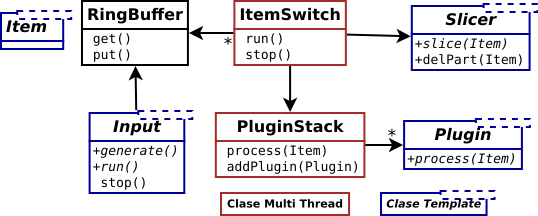
\includegraphics[width=\textwidth]{img/clasesFramework.pdf}

	\caption{Diagrama de clases Framework base.}

\end{figure}

Existen dos parámetros ajustables. El primero es la cantidad de hilos que
ejecutaran las tareas de búsqueda. El segundo parámetro es la cantidad de partes
en las cuales se dividirá el cuadro.

Para adaptar el framework para utilizarlo como un sistema de visión por
computadora para el fútbol de robots se incorporaron las siguientes clases, las
cuales fueron tomadas y modificadas del sistema de visión presentado en
\cite{torres2014}:

\begin{description}

\item[Frame:] Subclase de \emph{Item}. Contiene una imagen que representa un
	cuadro y una estructura auxiliar que contiene la información necesaria
	para el funcionamiento de los plugins.

\item[CaptureFromFile:] Subclase de \emph{Input}. Es la clase encargada de crear
	el flujo de objetos \emph{Frame}, tomando cada cuadro desde un archivo
	de vídeo.

\item[FastCaptureFromFile:] Subclase de \emph{Input}. Muy similar a
	\emph{CaptureFromFile}, con la diferencia de que carga los cuadros a
	memoria antes de que comience el sistema a capturar los cuadros. Esta
	clase fue creada para la experimentación, ya que leer el vídeo desde el
	disco en tiempo real introducía un retraso que no estaría presente si el
	vídeo se capturase de una cámara.

\item[FrameSlicer:] Subclase de \emph{ItemSlicer}. En este caso lo que se divide
	es la imagen del cuadro. Cada sub cuadro tendrá un solapamiento con los
	adyacente ya que se debe evitar que un robots o la pelota no este
	totalmente contenido dentro de por lo menos un sub cuadro. Para
	minimizar el área solapada, las particiones se realizan de manera tal
	que se minimice el perímetro pero ocupen la mayor área posible. Para
	lograr esto se busca la partición que haga que la relación entre el alto
	y el ancho sea lo mas cercana a uno.

\item[Subclases de \emph{Plugin}:] \emph{PluginBlur},
	\emph{PluginColorConversions}, \emph{PluginColorSegmentation},
	\emph{PluginDetectBalls}, \emph{PluginFindBlobs},
	\emph{PluginFindSecondariesBlobs}, \emph{PluginMorphology} y
	\emph{PluginNetworking}.

\item[Clases auxiliares:] \emph{ball}, \emph{colorspace}, \emph{datastruct},
	\emph{homography}, \emph{marker}, \emph{pattern},
	\emph{pattern\_matching}, \emph{practicalsocket}, \emph{segmentation},
	\emph{team}, \emph{timer}.

\end{description}

\begin{figure}[h]

	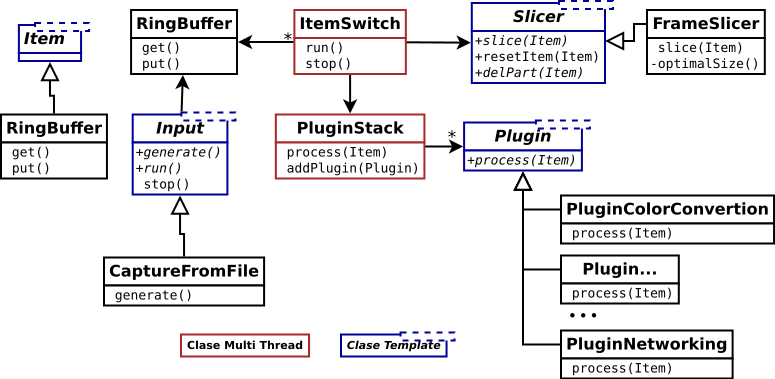
\includegraphics[width=\textwidth]{img/clasesFrameworkRobots.pdf}

	\caption{Diagrama de clases Framework del framework instanciado para el
	sistema de visión para el fútbol de robots.}

\end{figure}

Conceptualmente, la implementación para fútbol de robots tiene dos pilas, una
para búsqueda de robots y la otra para búsqueda de la pelota. Sin embargo, ambas
pilas para la etapa de pre procesamiento de la imagen utilizan los mismos
plugins con la misma configuración, ademas, los plugins que no tienen en común
solo modifican datos propios de cada pila. Esto permite que ambas pilas puedan
ser unidas en una sola, lo que trae como ventaja que la etapa de pre
procesamiento se realice solo una ves por cuadro.
